\section{Results}
\label{sec:results}

\placeholder{remaining exploratory numbers}{E17, E18, E19 (laser anchors) and E20 are confirmatory. Orange numbers are exploratory (\cref{sec:experiments}): the motivation numbers of \cref{sec:res:failure} beyond \cref{tab:main}, the probe-count ablation, and E19 with iPad anchors; E19 table cells are still rendered orange.}

%% ---------------------------------------------------------------- Table 2 (NYU/KITTI)
\begin{table}[t]
\centering\footnotesize
\setlength{\tabcolsep}{3pt}
\newcommand{\rowE}[3]{#1 & #3 & \ESeventeen{#2}{#3}{local} & \ESeventeen{#2}{#3}{dual} & \ESeventeen{#2}{#3}{short} & \ESeventeen{#2}{#3}{dW} & \ESeventeen{#2}{#3}{bW} & \ESeventeen{#2}{#3}{dIS} & \ESeventeen{#2}{#3}{bIS} \\}
\begin{tabular}{@{}llccccccc@{}}
\toprule
 & & \multicolumn{2}{c}{Coverage} & Short (\%) & \multicolumn{2}{c}{$\Delta$ width (\%)} & \multicolumn{2}{c}{$\Delta$ IS (\%)} \\
\cmidrule(lr){3-4}\cmidrule(lr){5-5}\cmidrule(lr){6-7}\cmidrule(l){8-9}
Layout & $k$ & \textsf{local} & \textsf{dual} & \textsf{dual} & \textsf{dual} & \textsf{both} & \textsf{dual} & \textsf{both} \\
\midrule
\rowE{uniform}{uniform}{50}\rowE{}{uniform}{200}
\midrule
\rowE{rows}{rows}{50}\rowE{}{rows}{200}
\midrule
\rowE{cluster}{cluster}{50}\rowE{}{cluster}{200}
\midrule
\rowE{edges}{edges}{50}\rowE{}{edges}{200}
\midrule
\rowE{near}{near}{50}\rowE{}{near}{200}
\midrule
\multicolumn{2}{@{}l}{theory} & $\ge$0.9$^\dagger$ & \NumDualCovTheory & \NumBetaShortOneTwenty$^\ddagger$ & & & & \\
\bottomrule
\end{tabular}
\caption{\textbf{NYU and KITTI, three frozen models, $n=20$ probes, $\alpha=0.1$}; confirmatory, \NumReplSplits{} scene splits $\times$ \NumProbeDraws{} probe draws; median over the six model--dataset pairs (ranges in the supplement). \textsf{local}: \mLocal calibrated on the $k$ structured anchors themselves; \textsf{dual}: \mDual; \textsf{both}: \mDualBoth. Short: \% of images whose coverage on one probe draw is below 0.85. $\Delta$: change in median relative width and relative interval score (IS, primary) against \mDistBoth. $^\dagger$Uniform anchors only. $^\ddagger$\Cref{tab:budget}.}
\label{tab:main}
\end{table}

%% ---------------------------------------------------------------- Figure 3
\begin{figure}[t]
\centering
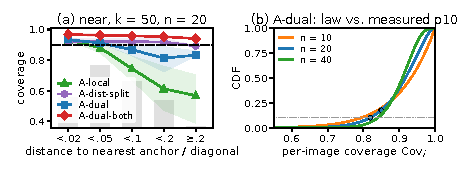
\includegraphics[width=\linewidth]{figures/e17_results.pdf}
\caption{\textbf{What each guarantee protects.} (a)~Near layout, $k=50$, $n=20$: \mDual's coverage decreases with distance, as \cref{thm:dual} allows; \mDualBoth is flat. Lines/bands: median/range over the six NYU/KITTI pairs; bars: pixel share; dashed: 0.9. (b)~CDF of the per-image coverage law (\cref{prop:budget}), $n=10,20,40$; dots at 0.1: measured p10 of $\Cov_i$ (median over pairs, layouts, $k$); dot at 0.85: measured share of short images, $n=20$. Confirmatory for $n=20$ (\NumReplSplits{} splits $\times$ \NumProbeDraws{} draws); $n=10,40$ exploratory.}
\label{fig:results}
\end{figure}

\subsection{Structured anchors break reused calibration}
\label{sec:res:failure}
Calibrating within the image on the structured anchors themselves (\cref{tab:main}, \textsf{local}) keeps nominal coverage only for uniform anchors.
Under clustered anchors it covers \ESeventeen{cluster}{50}{local} and \ESeventeen{cluster}{200}{local} at $k=50$ and $200$, under near-only anchors \ESeventeen{near}{50}{local} and \ESeventeen{near}{200}{local}, and under scan lines \ESeventeen{rows}{200}{local} at $k=200$; edge anchors over-cover, since edges are where errors are largest.
The failing intervals are narrower, not wider: with 20 clustered anchors their median relative width was \NumLocalClusterWidthLo--\NumLocalClusterWidthHi{} against \NumLocalUnifWidthLo--\NumLocalUnifWidthHi{} for uniform ones.
Even uniform anchors hide a spatial gap: coverage fell from \NumLocalNearBinCovLo--\NumLocalNearBinCovHi{} next to an anchor to \NumLocalFarBinCovLo--\NumLocalFarBinCovHi{} beyond 0.2 of the diagonal.

\subsection{Separating the roles restores per-image validity}
\label{sec:res:dual}
\mDual covers \NumDualCovLo--\NumDualCovHi{} in every layout, $k$ and pair, at its theoretical rate $r/(n+1)=\NumDualCovTheory$ (within two standard errors in \NumDualExactCells{} of the \NumAllCells{} pair--layout--$k$ cells), and is at least 10\% narrower than \mDistBoth on \NumDualGatePairs{} of \NumPairs{} pairs in each of the \NumCells{} layout--$k$ cells (\cref{tab:main}; paired bootstrap intervals exclude 0).
Part of that width is \mDistBoth's over-coverage (\NumDistBothCovLo--\NumDistBothCovHi), so the interval score, which charges misses, is the fairer comparison.
On it \mDual is better in \NumDualISWins{} of the \NumAllCells{} cells, including every cell with uniform or scan-line anchors (by \NumDualISGainURLo--\NumDualISGainURHi\%); \mDistBoth is better in \NumDualISLosses, nine of them clustered, by at most \NumDualISLoseMax\%.
\mDualBoth is better than \mDistBoth in \NumDualBothISWins{} cells and worse in \NumDualBothISLosses, all clustered and by at most \NumDualBothISLoseMax\%; under clustered anchors its halves are centred differently and it gains only \NumDualBothClusterWidthLo--\NumDualBothClusterWidthHi\% in width.
\mDual's coverage varies across distance bins by \NumSpreadDualLo--\NumSpreadDualHi{} points; \mDualBoth reduces this to \NumSpreadDualBothLo--\NumSpreadDualBothHi{} (\cref{fig:results}a).

\subsection{The probe budget}
\label{sec:res:budget}
With 20 probes the 10th percentile of $\Cov_i$ was \NumMeasPTenTwenty{} (law: \NumBetaPTenTwenty) and \NumESeventeenShort{} of images were short in one draw (law: \NumBetaShortOneTwenty\%), an implementation check (\cref{fig:results}b).
With 10 probes \mLocalSplit, hence \mDistBoth, is infinite on every image (5 calibration probes, fewer than the 9 needed), while \mDual stays finite at median width \NumWDualTenFifty/\NumWDualTenTwoHundred{} ($k=50/200$).
In exploratory runs with 40 probes, the share of images short on average over two draws fell to \NumShortFortyLo--\NumShortFortyHi\% (law: \NumBetaShortTwoForty\%) at similar width (\NumWDualFortyFifty/\NumWDualFortyTwoHundred), but under clustered anchors \mDual misses the 10\% margin over \mDistBoth. We keep $n=20$.

%% ---------------------------------------------------------------- Table 3 (ARKitScenes, E19)
\begin{table*}[t]
\centering\footnotesize
\setlength{\tabcolsep}{2.5pt}
\newcommand{\eA}[3]{\ENineteen{#1}{#2}{clean}{clean}{#3}{cov} & \ENineteen{#1}{#2}{clean}{clean}{#3}{ptten} & \ENineteen{#1}{#2}{clean}{clean}{#3}{short} & \ENineteen{#1}{#2}{clean}{clean}{#3}{wgt} & \ENineteen{#1}{#2}{clean}{clean}{#3}{is}}
\newcommand{\rowA}[3]{#1 & #3 & \eA{uniform}{#2}{#3} & \eA{cluster}{#2}{#3} \\}
\newcommand{\eB}[3]{\ENineteen{#1}{#2}{clean}{clean}{#3}{cov} & \ENineteen{#1}{#2}{lidar}{clean}{#3}{cov} & \ENineteen{#1}{#2}{clean}{lidar}{#3}{cov} & \ENineteen{#1}{#2}{lidar}{lidar}{#3}{cov}}
\newcommand{\rowB}[3]{#1 & #3 & \eB{uniform}{#2}{#3} & \eB{cluster}{#2}{#3} \\}
\newcommand{\eC}[3]{\EEighteen{#1}{#2}{clean}{clean}{#3}{cov} & \EEighteen{#1}{#2}{lidar}{clean}{#3}{cov} & \EEighteen{#1}{#2}{clean}{lidar}{#3}{cov} & \EEighteen{#1}{#2}{lidar}{lidar}{#3}{cov}}
\newcommand{\rowC}[3]{#1 & #3 & \eC{uniform}{#2}{#3} & \eC{cluster}{#2}{#3} \\}
\ifenvelopemain
\newcommand{\envrow}{ & \mDualEnv & -- & -- & \pending{env} & \pending{env} & -- & -- & \pending{env} & \pending{env} \\}
\else
\newcommand{\envrow}{}
\fi
\textbf{(a) Laser-valued anchors and probes: which centre to calibrate}\\[2pt]
\begin{tabular}{@{}llccccc@{\hspace{5pt}}ccccc@{}}
\toprule
 & & \multicolumn{5}{c}{Uniform layout} & \multicolumn{5}{c}{Cluster layout} \\
\cmidrule(lr){3-7}\cmidrule(l){8-12}
Centre & Calib. & Cov. & p10 & Short\,\% & W$/y$ & IS & Cov. & p10 & Short\,\% & W$/y$ & IS \\
\midrule
UniDepthV2 & \mSplitCP & \eA{uniform}{unidepth}{split-CP} & \eA{cluster}{unidepth}{split-CP} \\
\midrule
\rowA{UniDepthV2 + $\cS$}{unidepth}{A-dist-split}
\rowA{}{unidepth}{A-dual}
\rowA{}{unidepth}{A-dual-both}
\midrule
\rowA{\omnidc + $\cS$}{omnidc}{split-CP}
\rowA{}{omnidc}{A-dist-split}
\rowA{}{omnidc}{A-dual}
\rowA{}{omnidc}{A-dual-both}
\midrule
\multicolumn{2}{@{}l}{theory, one draw} & \NumDualCovTheory & \NumBetaPTenTwenty & \NumBetaShortOneTwenty & & & \NumDualCovTheory & \NumBetaPTenTwenty & \NumBetaShortOneTwenty & & \\
\bottomrule
\end{tabular}\\[6pt]
\textbf{(b) Laser-truth coverage by value source of anchors / probes (L = laser, I = iPad LiDAR)}\\[2pt]
\begin{tabular}{@{}llcccc@{\hspace{14pt}}cccc@{}}
\toprule
 & & \multicolumn{4}{c}{Uniform layout} & \multicolumn{4}{c}{Cluster layout} \\
\cmidrule(lr){3-6}\cmidrule(l){7-10}
Centre & Calib. & L/L & I/L & L/I & I/I & L/L & I/L & L/I & I/I \\
\midrule
\rowC{UniDepthV2 + $\cS$}{unidepth}{A-dist-split}
\rowC{}{unidepth}{A-dual}
\rowC{}{unidepth}{A-dist-both}
\envrow
\midrule
\rowC{DA-V2 + $\cS$}{dav2}{A-dual}
\midrule
\rowB{\omnidc + $\cS$}{omnidc}{split-CP}
\rowB{}{omnidc}{A-dist-split}
\rowB{}{omnidc}{A-dual}
\bottomrule
\end{tabular}
\caption{\textbf{ARKitScenes, $k=200$ ($180$ structured anchors $+$ $20$ probes), $\alpha=0.1$.} (a) and the \omnidc rows of (b): E19, UniDepthV2 frozen, mean over \NumOmniSeeds{} visit splits, one probe draw (confirmatory; \omnidc with iPad anchors, I/L and I/I: exploratory, three splits). Frozen-model rows of (b): E18, mean over \NumReplSplits{} visit splits and \NumProbeDraws{} probe draws (confirmatory). Coverage is always of the laser ground truth. p10 and short: 10th percentile of per-image coverage and \% of images below 0.85, for a single probe draw. W$/y$: median width over laser depth; IS: relative interval score (\cref{sec:experiments}). \omnidc sees RGB and the structured anchors only, never the probes. \mSplitCP calibrates on dense laser depth of calibration scenes; \mDistSplit on the values the measurements report. Under clustered anchors, 0.1--0.4\% of \omnidc pixels with extreme upper bounds dominate a mean over images, not the IS shown (Supp.~G). Full grid in the supplement.}
\label{tab:arkit}
\end{table*}

\subsection{Which centre to calibrate}
\label{sec:res:omni}
\emph{Uniform anchors.} \omnidc is the better centre: \mSplitCP, \mDual and \mDistSplit on its output have a \NumOmniGainLo--\NumOmniGainHi\% lower interval score than \mDual on UniDepthV2 (paired intervals exclude zero), which fires the criterion we fixed before the run ($\ge$15\%), so the layer belongs on top of the completion network.
\mDual with \omnidc as centre costs \NumOmniDualCost\% in interval score over \mSplitCP on the same output and adds the per-image law: p10 \ENineteen{uniform}{omnidc}{clean}{clean}{A-dual}{ptten} and \ENineteen{uniform}{omnidc}{clean}{clean}{A-dual}{short}\% short images in one draw, as \cref{tab:budget} predicts.
\mSplitCP's spread is similar here (\ENineteen{uniform}{omnidc}{clean}{clean}{split-CP}{short}\% short) but carries no per-image guarantee, and it needs dense reference depth on calibration scenes.
\mDistSplit on \omnidc is the most efficient (\ENineteen{uniform}{omnidc}{clean}{clean}{A-dist-split}{is}) but has no per-image guarantee and, under uniform anchors, fails with sensor-valued anchors (\cref{sec:res:sensor}).
Without anchors, \mSplitCP on the frozen model has \NumRawRatioLo--\NumRawRatioHi$\times$ the interval score of any anchored method.

\emph{Clustered anchors.} The ranking reverses.
Away from one observed patch the completion network extrapolates poorly (AbsRel 0.074, vs.\ 0.039 for UniDepthV2 rescaled by the same anchors; Supp.~G): \mSplitCP on its output falls short of validity (coverage \ENineteen{cluster}{omnidc}{clean}{clean}{split-CP}{cov}, more than 2\,SE below 0.9) with p10 \ENineteen{cluster}{omnidc}{clean}{clean}{split-CP}{ptten} and \ENineteen{cluster}{omnidc}{clean}{clean}{split-CP}{short}\% short images, and \mDual on UniDepthV2 has a \NumClusterGainDual\% lower interval score than \mDual on \omnidc (\NumClusterGainCP\% lower than \mSplitCP on \omnidc, where \mDual beats \mSplitCP by 17\%).
The monocular prior carries the far field and the anchors fix its scale; this holds over \NumOmniSeeds{} splits, for one network and one dataset.
On this centre \mDistSplit is more efficient still (\ENineteen{cluster}{unidepth}{clean}{clean}{A-dist-split}{is}), without a per-image guarantee; \mDualBoth keeps both guarantees at \ENineteen{cluster}{unidepth}{clean}{clean}{A-dual-both}{is}.
Across both centres and layouts, \mDual's per-image spread is the same (p10 \NumENineteenPTenLo--\NumENineteenPTenHi, \NumENineteenShortLo--\NumENineteenShortHi\% short), as \cref{thm:dual} requires of any probe-independent centre.
\subsection{What the probes certify: an independent sensor}
\label{sec:res:sensor}
\Cref{tab:arkit}b (E18, confirmatory) varies what the measurements report, for UniDepthV2 and DA-V2 (AbsRel \NumArkUniAbsRel{} and \NumArkDavAbsRel) over \NumReplSplits{} visit splits $\times$ \NumProbeDraws{} draws, on data not used to choose $\gamma$.
With laser values for both, \mDual covers \NumEEighteenCovLL{} with the predicted spread.
With iPad anchors and laser probes, it covers the laser truth at \NumEEighteenCovIL{} in both layouts with the same spread (p10 \NumEEighteenPTen, short \NumEEighteenShort{} over both cells), because the probes measure the truth and absorb the anchors' bias into the threshold.
\mDistSplit, calibrated on the values the measurements report, covers it at only \NumEEighteenDistIpad{} under uniform anchors; its wider cluster bins absorb the bias (\NumEEighteenDistIpadCluster).
With laser anchors and iPad probes, \mDual over-covers (\NumEEighteenCovLI{} uniform, \NumEEighteenCovLICluster{} cluster), with \NumEEighteenWiden$\times$ wider intervals under uniform anchors, as the iPad's own errors enter the threshold.
With iPad values for both, the deployed configuration without a reference, \mDual certifies the iPad reading.
Under uniform anchors its intervals are about as narrow as the \NumArkIpadOffset\% sensor bias, and it covers the laser truth at only \NumEEighteenCovII{} (p10 \NumEEighteenPTenII, short \NumEEighteenShortII; \omnidc: \ENineteen{uniform}{omnidc}{lidar}{lidar}{A-dual}{cov}); the wider cluster intervals absorb more (\NumEEighteenCovIICluster), and the hull \mDualBoth recovers the truth there (\NumEEighteenHullIICluster) but not under uniform anchors (\NumEEighteenHullII).
Earlier within-image methods do the same (iPad anchors: \mLocal{} \NumArkLocalIpadCovUni, LSCP~\cite{jiang2024lscp} \NumArkLscpIpadCovUni).
Two methods cover the truth in every cell: \mSplitCP, because it calibrates on laser depth of other scenes, which a deployed system lacks, and \mDistBoth (at least \NumEEighteenDistBothMin) through width, at \NumEEighteenDistBothRatio$\times$ \mDual's interval score under uniform anchors with laser values.
Probes certify what they measure\ifenvelopemain; sensor-grade probes need \cref{sec:env}.

\placeholder{envelope, not yet run}{fills the \mDualEnv row; if the gate fails, set \texttt{\textbackslash envelopemainfalse}.}
\else.
The envelope of Supp.~D restores truth coverage with iPad probes (\NumEnvTruthCov) but over-covers, at an interval score \NumEnvISWorse{} above \mDistBoth's.
\fi
